% -*- coding: utf-8; -*-
\documentclass[a4paper]{report}

%%%% LANGUAGE
\usepackage{geometry}       % marges
\usepackage[utf8]{inputenc}
\usepackage[T1]{fontenc}
\usepackage[english]{babel}
\usepackage{setspace}
\usepackage{microtype}
\usepackage{lmodern}
\usepackage{graphicx}
%%%% STRUCTURE
\usepackage{caption}
\usepackage{subcaption}
\usepackage[plainpages=false, colorlinks=true, linkcolor=black,
urlcolor=MidnightBlue]{hyperref}
\usepackage{enumitem} % For nested list like 1.2.2

%%%% COLORS
\usepackage{fancyvrb}
\usepackage[usenames,dvipsnames]{xcolor}

%%%% Formating
\usepackage{verbatim}
\usepackage{pdfpages} % pour insérer des pages PDF
\usepackage{listings}

% COMMANDS
% For writing inline code
\newcommand\code[1]{\texttt{#1}}

\newcommand\courriel[1]{%
  \href{mailto:#1}{\nolinkurl{#1}}%
}%

\newcommand{\source}[1]{%
  \nobreak\parbox[t]{\linewidth}{\raggedleft #1}% Placing a quote source
}%


\def\mytitle{On-Set Reconstruction Tool}

\title{\mytitle}

\def\myauthor{Louis Viot, Matthieu Pizenberg, Arthur Manoha, Nicolas
  Gaborit, Matthias Benkort}
\author{\myauthor}

\date{From January, 19\up{th} to March, 13\up{th}}

\begin{document}

\begin{titlepage}
\centering

\null
\vfill

{\Huge\sffamily\bfseries\mytitle\par}
\vspace{1cm}
{\Large\myauthor\par}

\vfill
\vfill


\includegraphics[width=5cm]{img/inpn7.pdf}

\vfill

{\Large \emph{Projet long} Final Report -- 2015\par%
  Clients : Simone Gasparini, Fabien Castan\par}


\end{titlepage}

\newpage

\thispagestyle{empty}
\null
\vfill

\section*{Acknowledgments}
Merci à tous

\chapter{Project overview}
\section{Objectives}
During this project, we have been leading to develop a Graphical User Interface 
which holds in background a complex processus pipeline. It aims at making automatic
and easier a common reconstruction process, used in the cinema industry in order
to compute \textsc{3d} models from a set of \textsc{2d} pictures. In the context
of the european project \emph{Popart},  we are trying to set up a small prototype
that may be shown as a proof of concept during further presentations of the project.

\noindent
Ensuring a global pipeline, we have also implemented as many as possible features
to enhance the completeness of the application. The whole application has been
developed using \code{python}, \code{C++} and \code{Qml} and various libraries 
and framework described in a related document. 

\noindent 
On the other hand, the project was a real opportunity to face and cope with 
management challenges. Well above the technical and practical experience we've get, 
we have learnt a lot about task managing, continuous risks analysis and scheduling.
The project ought to give us an overview of future situations we may encounter.  

\section{Supplies}
The core of the application relies on a specific reconstruction library called 
\emph{openMVG}. It is indeed an essential cornerstone of the project; it has 
been supplied by the client via a \emph{GitHub} repository. Given that, various 
indications were offered either about languages to use or useful libraries.

\section{Deliverables}
As a product, we delivered our prototype version in the form of a \emph{GitHub} 
repository. In that way, client is able to clone the repository and launch the 
application from a defined milestone. Plus, he might be able to carry on our 
work by taking the lead onto this repository. 
Also, the repository allow us to gather source code on one side, and a documentation
on the other side. The documentation is by the by compiled into \code{html} 
documents and it is therefore easily accessible online. 



\chapter{Project Management}
\section{Team and Roles}

Our team  is comprised of:
\begin{itemize}
\item Arthur Manoha
\item Louis Viot
\item Matthias Benkort
\item Matthieu Pizenberg
\item Nicolas Gaborit
\end{itemize}


We defined three specific roles within our team. These are the project
manager, the technical manager and the integration manager.

\begin{description}
\item[Technical Manager] \emph{(Matthias Benkort)} He is the one who
  has to know best the technologies we are using because he serves as
  a technical reference for the rest of the team. He is responsible
  for the overall architecture of the application and validates
  choices made in this regard. He is responsible for the overall
  quality of the code, including its extensibility and re-usability. He
  also insure the overall consistency of the code by defining early on
  some coding style rules in a document called: Coding Style Guide.

\item[Integration Manager] \emph{(Matthieu Pizenberg)} He is the
  central part, insuring the code developed by everyone integrate well
  together without adding bugs. He setups the development environment
  (Git) and defines an integration process and a development work flow
  for this purpose. He is available to help everyone with the
  development tools.

\item[Project Manager] \emph{(Arthur Manoha then Nicolas Gaborit on
    week 5)} He is the team coordinator. He ensures good communication
  with the client and within the team. He establishes the planning and
  manage its evolution with the team. He also make sure a proper risk
  analysis is regularly made.
\end{description}


\section{Meetings}
We had two types of meeting throughout the project, the first with the
clients and the second with the industrial supervisor.

\subsection{Clients}
We met every Friday with the clients to present our progress, ask some
questions about problems we are facing or choices we are making, and
get a feedback from them. They lasted one hour and a half. However,
we tried not to wait until Friday when we needed to clarify things and
thus we used mails or video calls to communicate outside of this
schedule.

\subsection{Industrial Supervisor}
Every Tuesday was our weekly review with the industrial
supervisor. During those we reported on our progress and
difficulties. In particular, we discussed the hows and whys of tasks
related to project management : planning, specifications, risks and
response plan.

\section{Development environment}
The project we work on is going to be resumed by POPART team
at the end of "projet long". Therefore we should have a clean workflow,
compatible with the POPART team one.\\

\noindent
To help us in that task we decided to use Git which allow to have
a fine control of the production flow.
Nevertheless not everyone knows how to use Git.
Thus, as a preliminary task we wrote two guides (annexed to this document) :
\begin{itemize}
  \setlength\itemsep{0em}
  \item Git Introduction
  \item Workflow for the "Projet Long" POPART
\end{itemize}

\noindent
Broadly speaking, we followed a mix of two classic workflows :
\begin{itemize}
  \setlength\itemsep{0em}
  \item \textbf{The Integration Manager workflow :}
    Each developer has its own fork of a blessed repository
    (which we call in our project "ref" for reference).
  \item \textbf{The Gitflow workflow :}
    A project is composed of two main branches (master and develop)
    and of many other supporting branches (features, releases, hotfix).
\end{itemize}

\noindent
Regarding the software and libraries needed,
they are too many and varying to list them here.
But they all are open source and available online.
You will find a more complete description of these
tools in the INSTALL.md file of our Github repository.

\section{Quality insurance}
This is a major black spot in our project.
We intended to produce high-quality code but we did not
setup a test environment. This due to a lack of time
at the end of the project.\\

\noindent
In the early stage of the project, along with the development environment,
we intended to setup a continuous integration and test environment based
on Github.
The idea was to use Travis (as a Github extension) to automatically launch
tests whenever new commits where pushed on the reference repository.
In addition we would have used Coverall (also as a Github extension)
to compute code coverage of our tests.\\

\noindent
In the end the only tests we have done are manual tests
quickly done before accepting pull requests in order to check
new functionality.
However, due to the lack of automatic tests, we did not ensure
backwards compatibility.\\

\noindent
Nevertheless, we tried to produce a clean, readable, maintainable code.
From this perspective we wrote a coding style guide (annexed to that document).
It describes the general conventions we should try to respect in order to
reach consistency across the project.
Since it was done at a moment where we thought we shall code in C++,
it is thus focused on C++ style guide.

\section{Risks Management}
We made a formal risks analysis during the early weeks as a
brainstorming initially. We listed all the risks we could think of and
sorted them according to both their probability and impact. Then we
decided of a response plan or solution for each of them. This first
risks analysis is fully visible on page \pageref{fig:risks}. However,
we did not reiterated this process later. 

This resulted in some unexpected problems whose main consequences were
to add delay to the project:

\begin{description}
\item[No 3D optimization in Python] The Python OpenGL bindings would
  not allow us to optimize the 3D rendering of the point cloud using
  \code{Vertex Array Objects} and \code{Buffer Objects}. So we needed
  to use \verb!C++! and make a QML plugin that could integrate in
  PyQt. Learning how to integrate a \verb!C++! plugin in PyQt took some time.
\item[Libraries installations] We tried to install the libraries we
  were using at the ENSEEIHT to allow everyone to work
  together. However it ended not being possible and some members of
  the team lost a few days in the process. We could have avoided that
  by analyzing first the risk involved and according us a deadline for
  the installations.
\end{description}

We did take some preventive actions though, but we did not formalized
it. For example, when we faced the necessity of using \verb!C++! Qt instead
of PyQt to develop the point cloud rendering QML plugin, we were not
certain of achieving this task in time. For this purpose, we developed
in parallel another faster, less satisfying solution.


\begin{figure}[!htbp]
  \centering
  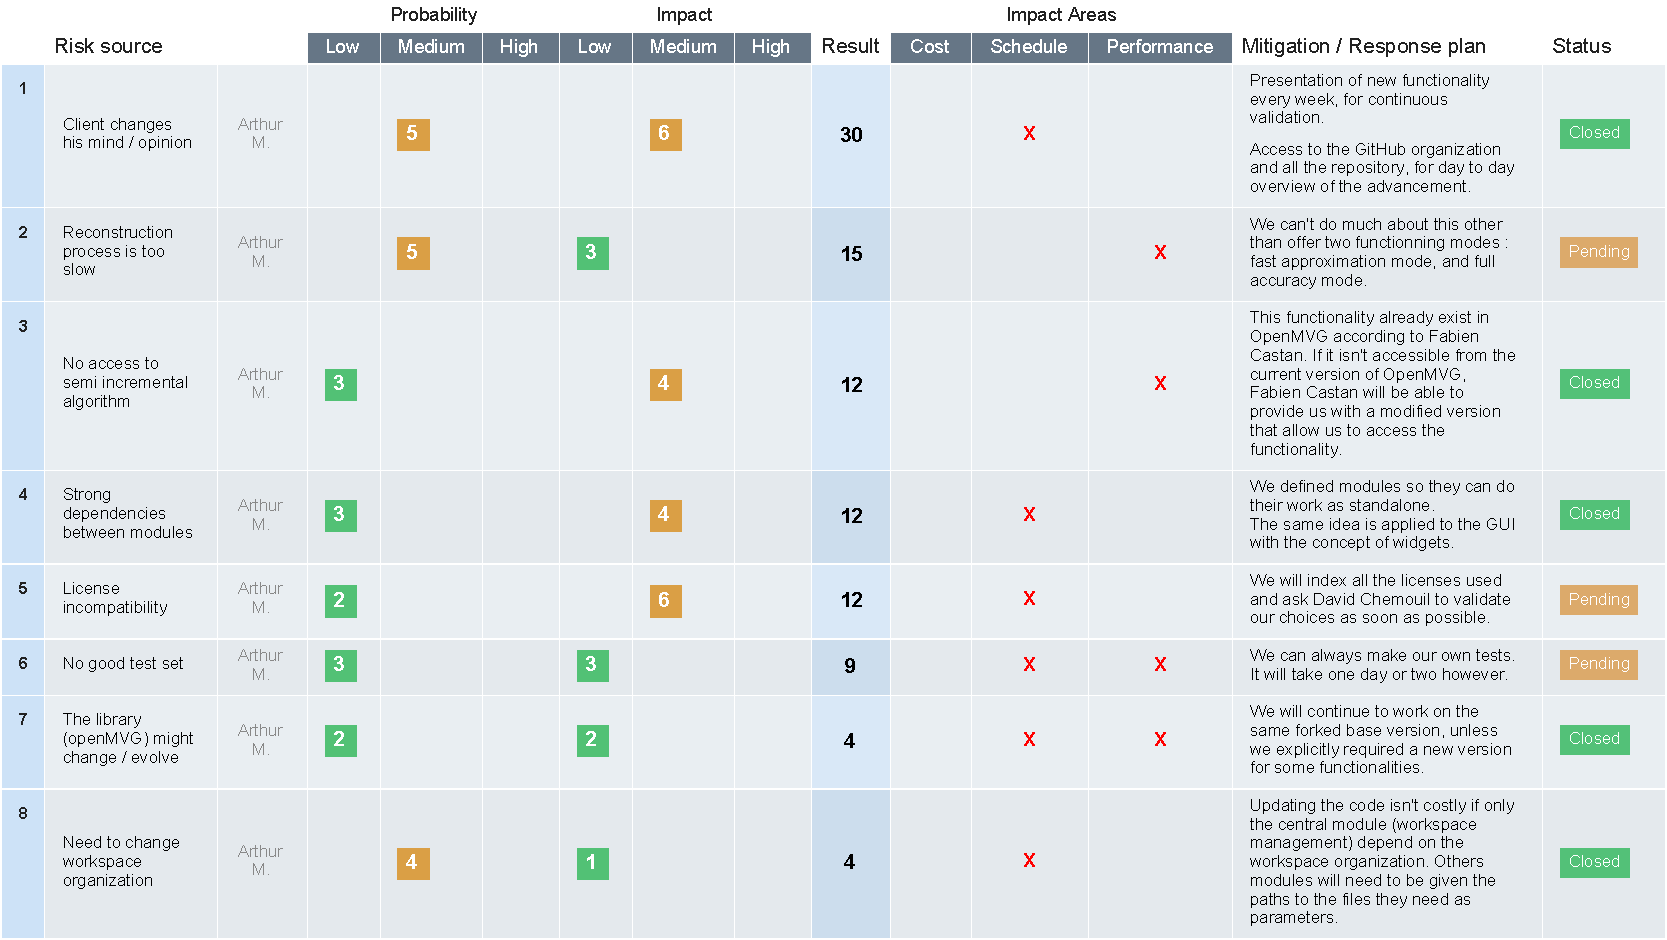
\includegraphics[width=\linewidth]{img/risks.pdf}
  \caption{Risks report on 3rd week}
  \label{fig:risks}
\end{figure}

\section{Planning}

Establishing a planning was the hardest project management task in the
project. First because we lacked the tools to work on PERT or Gantt
diagrams easily\ldots The one we used
(\href{https://www.teamwork.com/}{Teamwork}) was incomplete but we
figured it out too late. Second because we had so many technologies to
learn before knowing what we had to do. And that is indeed the point:
we should have planned our training period. The key is not to have a
fully detailed planning like the first one we came up with. The key is
to start small and refine the planning as the project goes. You will
find the planning we made on week 5 as an appendix on page
\pageref{app:planning}.


\chapter{Conclusions}
\section{Realized parts}
We will present in this section what is currently usable in the final version of the application.
\subsection*{Workspace Management}
When the user launch the application, he will be asked to create a new workspace. You cannot use the application without first creating a workspace, like in eclipse. 
When a workspace is created, in a specific folder, you can create another workspace, delete your current workspace or change to another workspace. When you are done with
a workspace, you can save it and re-open it later.

In a workspace, you can create a scene or multiple scenes. A scene corresponds to a set of photos, like a real scene. You can change your current scene to another one already created or delete your current scene. Note
that when you create a workspace, a default scene is created so you don't have to create a scene.

\subsection*{Pictures Handling}
When you are in your workspace, you can import pictures, either from a specific folder or from a camera. If a camera is connected, the application will detect it and display its name. If you choose to import photos from
your camera, the application will import \textbf{all} your photos as thumbnails. 

You can then manage your pictures, select the one you want to import as real photos and not as thumbnails by setting their state as \textit{Discarded} or \textit{New}, if you imported them from your camera. The is on 
the left of the screen a list with your pictures and a preview above the list. You can select pictures, drag and drop them as you want to sort them. You can filter them by their state.

\subsection*{Map View}
If you switch on the \textit{Show the map} button, a map centered on your pictures will appear (if you have pictures with GPS exif data, otherwise the map be centered on the point of coordinates 0.0,0.0). You can 
navigate on the map as you want, or click on a picture in the preview list to center the map on it. You can also click on a point on the map to select the corresponding picture in the list. Note that each picture state has
its own color code, see the documentation for further details. There is a good interaction between the preview list and the map. 

\subsection*{Reconstruction}
When you are all set for the reconstruction, meaning that you have selected a set of pictures you want to use for the recontruction, you can launch the 3D reconstruction. In the current version of the application,
this will freeze the application and you will have to wait for the reconstruction to be done to be able to re-use the application. Once the reconstruciton is done, you will see the 3D rendering of your scene wetween the map
and the preview list.

\subsection*{3D Renderer}
The 3D renderer currently only display a point cloud when the application gives him one. Note that the point of view from where you see the point cloud is the exact location of one of your camera. There 
are still not any interactions between the 3D renderer and the rest of the application, see the documentation for further details about that.

\section{Missing features}
While the application was supposed to be a prototype and was not to be a hundred percent usable and stable, there are still essentials features that are missing. Here a list of those features, classified by their importance :
\begin{description}
\item[Dynamic behavior between Pictures selection, Map view and 3D View] There are many interactions between the preview list and the map viewer like said previously. One important feature that evry user would naturally
expect is the same type of interaction between those two modules and the 3D view. Clicking on a picture would not only change the current view of the map, but also the current view on the 3D view.
\item[3D Navigation] Being able to navigate inside the 3D world to see the point cloud is also something any user would expect to be present in the application. 
\item[Automated Reconstruction] As said before, you have to manually launch the reconstruction when you have selected your pictures. What the client expected from us was that the application would automatically launch
a new reconstruction when a new picture, in the right state, has been added. 
\item[Reconstruction Feedback] When the user launches the reconstruction, he currently never knows if there are problems with the reconstruction, or its progress state. A feedback, simply like logs, is also something missing.
\end{description}

\section{Insights}
Here we will try to conclude and describe a bit our feelings about this project. The first question to be asked at the end of this project is : \textbf{Did we reach client expectations ?} . 
As said before, we implemented most of the functionalities we were asked to do, but some import features are still missing. But this project being our first big group project, we have encountered many isssues we did not expect
to encounter, and those issues made us late on what was initially schedueled. But we have learned from those issues and we are now stronger and more prepared for future projects we might have, and we think this is the 
main objective of the \textit{projet long}. And given the fact that none of use knew any of the languages used for the project and that the client knew about that, we can say that we have reached client expectations.

But, while reading this, one has to keep in mind that the main goal of this project was to build a prototype that our client could easily re-use for demonstration or for snippets of code. We have also build a solid 
architecture around the project, a good documentation which explain communications between modules of this architecture	and so we have proved that the application could be done. The application can now be re-used that way and is 
also extendable.




\appendix
\chapter{Specifications}
\chapter{Mockup}
\chapter{Workflow documents}
\chapter{Coding style guide}
\chapter{MATRIX's Documentation}
\chapter{Any other Google Doc ??}

\end{document}